\documentclass{article}
\usepackage[utf8]{inputenc}
\usepackage{amssymb}
\usepackage{graphicx}

\usepackage[lmargin=2.5cm,rmargin=2cm,tmargin=3cm,bmargin=2.5cm]{geometry}

\setlength{\parindent}{0pt}

\begin{document}

\section{Resolución de ecuaciones de recurrencia lineal de primer orden}

Una ecuación de recurrencia lineal de primer orden relaciona entradas consecutivas en una secuencia por una ecuación de la forma:

 $$S_{n+1}=a S_{n}+c \qquad\textit{ para todo n en el dominio de S}....(*)$$

Una solución general es una descripción algebraica de todas estas secuencias de soluciones.\\
Si S es cualquier secuencia en N que satisface la ecuación anterior, entonces denotando $S_0$ por I, tenemos:\\

\begin{tabular}{lll}
    $S_1 =$ & $aS_0 + c$  & $=aI+c$ \\
    $S_2 =$ & $aS_1 + c = a[aI + c]+c$  & $=a^2I+ac+c$ \\
    $S_3 =$ & $aS_2 +c = a[a^2 I +ac + c] + c$ & $=a^3I+a^2c+ac+c$\\
   \vdots & &
\end{tabular}

Entonces podríamos decir que:
$$S_n = a^nI + a^{n-1}c + a^{n-2}c + ... + ac + c \qquad \textit{para $\forall n \in \mathbb{P}$}.....(**)$$

Podemos demostrarlo por INDUCCIÓN MATEMÁTICA para cualquier $k \in \mathbb{P}$, $S_k = a^kI + a^{k-1}c + a^{k-2}c + ... + ac + c$, entonces:\\

\begin{tabular}{cl}
    $S_{k+1} = & aS_{k} + c  \\
    S_{k+1} = & a[a^kI+a^{k-1}c+a^{k-2}c + ... + ac +c] + c\\
    S_{k+1}= & a^{k+1}I + a^k c+a^{k-1}c + ... + a^2c+ ac + c$
\end{tabular}

Por lo tanto, (**)  es correcto. Por lo tanto, si S es cualquier secuencia en N que satisface (*), entonces para $\forall n \in \mathbb{P}$\\\\

Si $a =1$, $S_n = 1^n I + 1^{n-1}c + 1^{n-2}+...+1c+c = I + nc$ y \\
Si $a \neq 1$, $S_n = a^n I+a^{n-1}c + a^{n-2}c + .... + ac +c$\\
$= a^nI + c \frac{1-a^n}{1-a} = a^n I + \frac{c}{1-a} - a^n\frac{c}{1-a}$\\
$=a^n[1-\frac{c}{1-a}] + \frac{c}{1-a}$\\\\

Por lo tanto la solución general a la ecuación de recurrencia:
$$S_{n+1} = aS_n + c \qquad \qquad \forall n \in \mathbb{N}$$
Se da en dos partes:\\
\begin{tabular}{cll}
    $\textit{Si} a=1, & S_n = S_0 + nc & \forall n \in \mathbb{N}\\
     \textit{Si} a\neq 1& S_n = a^n [S_0 - \frac{c}{1-a}] + \frac{c}{1-a}  &\forall n \in \mathbb{N} $
\end{tabular}
 
 

\subsection{Las Torres de Hanoi}

Cuenta la leyenda que los monjes de un monasterio de Hanoi miden el tiempo que falta para la llegada del fin del mundo con elsiguiente procedimiento: Disponen de tres agujas de diamante, en una de las cuales se apilan 64 discos de oro distintos, ordenados por tamaños. Cada segundo mueven un disco de una aguja a otra, y su tarea finalizará (y con ella el mundo) cuando logren transportarlos todos a otra aguja. Pero, ¡atención!, a lo largo del proceso nunca se puede colocar un disco sobre otro de diámetro más pequeño.\\

Como prepararnos para el fin del mundo supondrá sin duda un notable ajetreo, vamos a estimar el tiempo de que dispondremos. Para ello, planteamos el problema ya en general: tenemos $n$ discos y llamamos $a_n$ al mínimo número de movimientos necesario para transportar los $n$ discos desde una aguja a otra.\\
Por ejemplo, $a_1 = 1$, porque nos basta con un movimiento para pasar el disco a otra aguja.\\
El cálculo de $a_2$ requiere ya un pequeño argumento: podemos, por ejemplo, pasar el disco pequeño a otra aguja, luego el grande a la tercera, para finalmente pasar el pequeño a esta tercera aguja, como en la figura:

\begin{figure}[h]
    \centering
    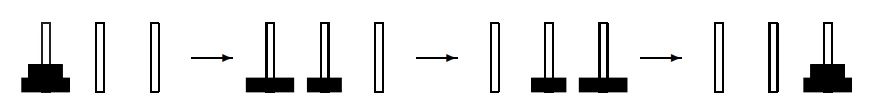
\includegraphics[scale=0.5]{real.jpg}
\end{figure}

Como en dos movimientos no se puede hacer, concluimos que la descrita es la mejor estrategia posible, y que, por tanto, $a_2 = 3$.\\

Si partimos de tres discos, podemos pasar los dos menores a una segunda aguja (con el procedimiento anterior, de tres movimientos), luego pasar el mayor a la tercera aguja, para finalmente llevar los dos discos menores sobre ese disco mayor (de nuevo tres movimientos). En total, 7 movimientos. Aunque ahora no está claro si se puede hacer el trasvase con menos.\\

El procedimiento esbozado en el caso $n=3$ se puede generalizar: si tenemos $n$ discos, pasamos $n-1$ a una segunda aguja, luego el mayor disco a la aguja final y, por último, pasamos los $n-1$ discos a esa tercera aguja. Es un algoritmo recursivo: el procedimiento para mover $n$ discos se apoya, dos veces, en el (ya conocido) método para mover $n-1$. Se deduce entonces que el número mínimo de movimientos para transportar $n$ discos cumple que

$$a_n \leq 2a_{n-1} + 1 \textit{   para cada } n \geq 2 $$
porque con $2a_{n-1} + 1$ movimientos lo sabemos hacer. Obsérvese que no es una ecuación de recurrencia, sino una desigualdad. Pero lo que nos gustaría es comprobar que, en realidad, la
relaci´on se cumple con un $=$ en lugar de un $\leq$. Desuciríamos así que muestra estrategia de movimientos es la mejor posible. Esto requiere un argumento extra.\\

Veámoslo: si tenemos $n$ discos, en algún momento tendremos que mover el disco mayor, para lo que necesitaremos haber llevado el resto de los discos a otra aguja, pues debe quedar una aguja libre. Esto requiere, como mínimo $a_{n-1}$ movimientos. Una vez movido el disco grande a una aguja, tendremos que mover los restantes $n-1$ discos sobre él, y esto exige, al menos, otros $a_{n-1}$ movimientos (sea cual sea la estrategia que empleemos). Así que 

$$a_n \geq 2a_{n-1} + 1$$
para $n \geq 2$. Reuniendo ambas condiciones, ya podemos afirmar que, para cada $n \geq 2$,

$$a_n = 2a_{n-1} + 1$$

La condición inicial ya la hemos visto, es $a_1 = 1$. La resolvemos por simple aplicación repetida de la regla de recurrencia:\\

$a_n = 2 a_{n-1} + 1 = 2(2_{n-2} + 1) +1 = 2^2 a_{n-2} +2 +1 = 2^2(2a_{n-3}+1) +2+1$

$a_n = 2^3 a_{n-3} + 2^2 + 2 +1 =2^3 (2a_{n-4}+1)+2+1 = 2^4 a_{n-4} + 2^3+2^2+2+1$

$a_n = \cdot = 2^{n-1}a_1 + 2^{n-2} + 2^{n-3} + \cdot 2 + 1 = \sum_{j=0}^{n-1}2^j = \frac{1-2^n}{1-2} = 2^n - 1$

Del caso $n=64$ deducimos que el fin del mundo llegará dentro de $a_{64}= 2^{64} -1$ segundos, esto es, ¡más de medio billón de años! Parece que, después de todo, la profecía de los monjes de Hanoi no debería ser una de nuestras mayores preocupaciones.

Podemos resolverlo segun la definición mencionada, tenemos
La ecuación de recurrencia para el número de movimientos en las Torres de Hanoi es una ecuación de recurrencia lineal de primer orden:
$$S_n = 2 S_{n-1} + 1$$

Sea $a=2$ y $c=1$, entonces $\frac{c}{1-a} = \frac{1}{1-2} = -1$, y cualquier secuencia $S$ que satisfaga esta relacion de recurrencia está dado por la fórmula\\

\begin{tabular}{cl}
   ${\bf T_{n}} =$  & $2^{n}[I - (-1)] + (-1)$ \\
    ${\bf T_{n}} =$ & $2^{n}[I + 1] - 1$
\end{tabular}\\
De la condición inicial tenemos $I=S_0=0$\\
 $\Rightarrow {\bf S_n} = 2^{n}[0+1] - 1 = 2^n -1$ 


\subsection{Los tres piratas naufragados}

Un barco pirata es naufragado en una tormenta en la noche. Tres de los piratas sobreviven y se encuentran en una playa la mañana después de la tormenta. Aceptan cooperar para asegurar su supervivencia. Ellos divisan a un mono en la selva cerca de la playa y pasan todo ese primer día recogiendo una gran pila de cocos y luego se van a dormir exhaustos.\\
Pero ellos son piratas.\\
El primero duerme bien, preocupado por su parte de los cocos; despierta, divide la pila en 3 montones iguales, pero encuentra uno sobrante que arroja en el arbusto para el mono, entierra su tercero en la arena, amontona los otros dos montones, y se va a dormir profundamente.\\
El segundo pirata duerme bien, preocupado por su parte de los cocos; se despierta, divide la pila en 3 montones iguales, pero encuentra uno sobrante que arroja en el arbusto para el mono, entierra su tercero en la arena, amontona los otros dos montones, y se va a dormir profundamente.\\

El tercero también duerme bien, preocupado por su parte de los cocos; despierta, divide la pila en 3 montones iguales, pero encuentra uno sobrante que arroja en el arbusto para el mono, entierra su tercero en la arena, amontona los otros dos montones juntos, y se va a dormir profundamente.\\

A la mañana siguiente, todos se despiertan y ven una pila algo más pequeña de cocos que se dividen en 3 montones iguales, pero encuentran uno sobrante que tiran en el arbusto para el mono.\\

{\bf ¿Cuántos cocos recolectaron el primer día?}\\

Sea $S_{j}$ denota el tamaño de la pila después del pirata $j$ y sea $S_{0}$ será el número que recogieron en el primer día. Entonces

$$
S_{0} = 3x+1 \textit{para algún número entero}\; "x" \; \textit{y} \; S_1 = 2x,
$$

$$
S_{1} = 3y+1 \textit{para algún número entero}\; "y" \; \textit{y} \; S_2 = 2y,
$$

$$
S_{2} = 3z+1 \textit{para algún número entero}\; "z" \; \textit{y} \; S_3 = 2z,
$$

$$\textit{y} \;\;
S_{3} = 3w+1 \textit{para algún número entero}\; "w".
$$

//¿Hay una ecuación de recurrencia aquí?

$$
S_{1} = 2x \; \textit{donde}\; x=(S_{0}-1)/3, \; \textit{entonces} \; S_{1} = (2/3)S_0 - (2/3);
$$

$$
S_{2} = 2y \; \textit{donde}\; y=(S_{1}-1)/3, \; \textit{entonces} \; S_{2} = (2/3)S_1 - (2/3);
$$

$$
S_{3} = 2z \; \textit{donde}\; z=(S_{2}-1)/3, \; \textit{entonces} \; S_{3} = (2/3)S_2 - (2/3).
$$

La ecuación de recurrencia satisfecha por los primeros $S_{j}$ es

\begin{equation}
    S_{j+1} = (2/3)S_{j} - (2/3)
\end{equation}

Si ahora tenemos $S_{4}=(2/3)S_{3}-(2/3), \textit{entonces} \; S_{4}=2[S_{3}-1]/3 = 2w$ para algún número entero $w$.\\

Queremos saber qué valor (o valores) de $S_0$ producirá un número entero par para $S_4$ cuando aplicamos la ecuación de recurrencia (1).\\

En (1), $a=2/3$ y $c=-2/3$, entonces $c/(1-a) = -2$, y así la solución general de (1) es

$$
S_{n}= (2/3)^{n}[S_0 + 2] -2
$$

Por lo tanto, $S_{4} = (2/3)^{4}[S_0+2]-2 = (16/81)[S_0 + 2]-2$ \\

$S_4$ será un número entero\\
$\Leftrightarrow S_{4} + 2$ es (un aún) el número entero\\
$\Leftrightarrow$ 81 divide en $[S_0 + 2]$\\
$\Leftrightarrow [S_0 + 2] = 81k$ para algún número entero $k$\\
$\Leftrightarrow S_0 = 81k - 2$ para algún número entero $k$.\\

$S_{0}$ debe ser un número entero positivo, pero hay un número infinito de respuestas posibles:

$$79\; o \;160 \; o \; 241\; o \; 322 \; o\; ...$$

//Necesitamos más información para determinar $S_0$.\\

//Si nos hubieran dicho que el primer día los piratas recolectaron entre 200 y 300 cocos, ahora podríamos decir que "el número que recogieron el primer día fue exactamente 241."


\subsection{Interés Compuesto}

Supongamos que se le ofrecen dos planes de ahorro para la jubilación. En el Plan A, empiezas con \$1,000, y cada año (en el aniversario del plan), te pagan un 11\% de interés simple, y agregas \$1,000.En el Plan B, empiezas con \$100, y cada mes, te pagan una-duodécima parte del 10\% de interés simple (anual), y agregas \$100.¿Qué plan será más grande después de 40 años?.\\
//¿Podemos aplicar una ecuación de recurrencia?\\
Considere el Plan A:\\
Sea $a_n$ denote el número de dólares en el plan después de (exactamente) $n$ años de operación. Entonces 
$a_0 = \$1,000$ y
$$S_{n+1} = S_{n} + \textit{interes sobre}\; S_n + \$1000$$
$$S_{n+1} = S_{n} + 11\% \textit{de} S_n + \$1000$$
$$S_{n+1} = S_{n}(1+0.11) + \$1000.$$

En esta ecuación de recurrencia, sean $a=1.11$, $c=1000$, entonces $\frac{c}{1-a}=\frac{1000}{-0.11}$. y 

$$S_{n}= (1.11)^{n} \left[1000 - \frac{1000}{-0.11}\right] + \frac{1000}{-0.11}$$
$$S_{n}=(1.11)^{n}\left[\frac{1110}{0.11}\right]- \frac{1000}{0.11}$$

Por lo tanto,\\
$S_{40} = (1.11)^{40}\left[\frac{1110}{0.11}\right]- \frac{1000}{0.11} \\
S_{40}=(65.000867...)(10090.090909...)-(9090.909090...)\\
S_{40}=655917.842...\; - \; (9090.909090...)\\
S_{40} \approxeq \$646826.$ \\

%//¿Puede ser cierto? Pusiste $40,000 y sacaste > $600,000 en intereses.\\

Ahora considere el Plan B:\\
Sea $T_n$ denota el número de dólares en el plan después de (exactamente) $n$ meses de funcionamiento. Entonces $T_0 = \$100$ y

$$T_{n+1} = T_{n} + \textit{interes sobre} T_{n} \;\; + \$100$$
$$T_{n+1} = T_{n} + (1/12) \textit{de}\; 10\% \textit{de}\; T_{n} + \$100$$
$$T_{n+1} = T_{n}[1+0.1/12] \;\; \$100$$

En esta ecuación de recurrencia, sean $a=12.1/12, c=100$, entonces $\frac{c}{1-a} = \frac{100}{-0.1/12} = -12000$ y

$$T_n = (12.1/12^{n})\left[100 - \frac{100}{-0.1/12}\right] + \frac{100}{-0.1/12}$$
$$T_n = (12.1/12)^{n}[100 + 12000] - 12000$$

De ahí, después $40x12$ meses,\\

$
T_{480}=(12.1/12)^{480}(12100) \;\; -(12000)\\
T_{480}=(1.008333...)^{480}(12100)\;\; -(12000)\\
T_{480}=(53.700663...)(12100)\;\; -(12000)\\
T_{480}=649778.0234... \;\; -(12000)\\
T_{480}\approxeq \$637778.
$\\
Por lo tanto, el Plan A tiene un valor ligeramente mayor después de 40 años.

\section{Resolución de ecuaciones de recurrencia lineal de segundo orden}



Una ecuación de la recurrencia lineal del segundo-orden relaciona entradas consecutivas en una secuencia por una ecuación de la forma

\begin{equation}
  S_{n+2} = aS_{n+1} + bS_{n} + c \;\; \forall\; n \; \textit{en el dominio de} \; S
\end{equation}

Pero vamos a asumir que el dominio de S es \mathbb{N}. Supongamos también que ni "a" ni "b" son 0; de lo contrario, $S_n = c$ para $\forall n \in  \{2.. \}$, y las soluciones para (2) no son muy interesante.\\

%// ¿Qué es de ellos?\\
La ecuación de recurrencia de primer orden son sólo un caso especial de la ecuación de recurrencia de  segundo orden  cuando $b = 0$.\\

Cuando $c = 0$, se dice que la RE es homogénenea (todos los términos se ven igual – una constante veces una entrada de secuencia).\\

La ecuación de recurrencia de Fibonacci es homogéneneo. \\

Vamos a restringir también nuestra atención (por el momento) a una ecuación de segundo orden lineal, la recurrencia homogénea

\begin{equation}
S_{n+2} = aS_{n+1} + bS_{n}\;\; \textit{para} \;\; \forall\; n \in \mathbb{N}
\end{equation}

Tal como hicimos para la ecuación de la recurrencia de Fibonacci, supongamos que hay una secuencia geométrica, $S_n = r^n$ , que satisface (3)\\

Si hubiera; entonces $r^{n+2} = ar^{n+1} + br^{n}$ para $\forall \; n \in \mathbb{N}$.\\

Cuando $n = 0$, \;\;\; $r^2 = ar + b$.\\

La "ecuación caractreristica" de (3) es $x^2 -ax-b=0$,\\

que tiene "raíces" $r = \frac{-(-a) \pm \sqrt{(-a)^2 - 4(1)(-b)}}{2(1)} = \frac{a \pm \sqrt{a^2 + 4b}}{2}$\\

Sea $\Delta = \sqrt{a^2 + 4b}$, $r_1 = \frac{a + \Delta}{2}$, y $r_2 = \frac{a - \Delta}{2}$.\\

Entonces $r_1 + r_2 = a$, $r_1 \textit{x} r_2 = -b$, y $r_1 - r_2 = \Delta $ \\

Tanto $r_1$ como $r_2$ satisfacen la ecuación $x^2 = ax + b$, y son las únicas soluciones.

\subsection{Ejemplo.}
Si $S_{n+2} = 10S_{n+1} - 21S_n$ para $\forall n \in \mathbb{N}$, la ecuación característica es $x^2 - 10x +21 = 0$.\\
//O $(x-7)(x-3)=0$\\
Donde, $a=10$, $b=-21$, $a^2+4b=100-84=16$, $\Delta = 4$, entonces $r_1 = 7$ y $r_2 = 3$.

\subsection{Ejemplo.}
Si $S_{n+2} = 3S_{n+1}-2S_{n}$ para $\forall \; n \in \mathbb{N}$, la ecuación caraterística es $x^2-3x+2=0$.\\
//O $(x-2)(x-1)=0$\\
Donde, $a=3$, $b=-2$, $a^2+4b=9-8=1$, $\Delta = 1$, entonces $r_1=2$ y $r_2=1$.


\subsection{Ejemplo.}
Si $S_{n+2} = 2S_{n+1}- S_{n}$ para $\forall \; n \in \mathbb{N}$, la ecuación caraterística es $x^2-2x+1=0$.\\
//O $(x-1)(x-1)=0$\\
Donde, $a=2$, $b=-1$, $a^2+4b=4-4=0$, $\Delta = 0$, entonces $r_1=1$ y $r_2=1$.\\\\


¿Pero qué hay de una fórmula que da la solución general?

\subsection{Teorema.}
//La solución general de la RE homogénea (3) es\\

$S_n = A(r_1)^n + B(r_2)^n$ si $r_1 \neq r_2$, \;\;\;\;\;\;\;\;\;\;\; //Si $\Delta \neq 0$\\
$S_n = A(r)^n + Bn(r)^n$ si $r_1 = r_2 = r$, \;\;\;\;\;\;\;\;\;\;\; //Si $\Delta = 0$\\

Prueba. Supongamos que T es cualquier solución particular de la RE homogénenea\\
// Nos ocupamos de los dos casos por separado.\\

Caso 1. Si $\Delta \neq 0$, entonces las dos raíces son distintas (pero pueden ser números "complejos").\\

// Encontraremos valores para A y B, luego probaremos que $T_n = A(r_1)^n + B(r_2)^n$ para $\forall n \in \mathbb{N}$\\
// Mostraremos $A(r_1)^n + B(r_2)^n$ arranca correctamente para valores especialmente elegidos\\
// de A y B, y luego mostrar $A(r_1)^n + B(r_2)^n$ continúa correctamente.\\

Vamos a resolver las ecuaciones (para A y B) que garantizaría $T_n = A(r_1)^n + B(r_2)^n$ entonces $n=0$ y $n=1$. Si\\

$T_0 = A(r_1)^0 + B(r_2)^0 = A + B$.................................(1)\\
 y $T_1 = A(r_1)^1 + B(r_2)^1 = A(r_1) + B(r_2)$.................................(2)\\
 
entonces $(r_1)T_0 = A(r_1) + B(r_1)$.......................//multiplicamos (1) por $r_1$\\
y $T_1 = A(r_1) + B(r_2)$.................// (2) otra vez restamos, obtenemos\\

$(r_1)T_0 - T_1 = B(r_1 - r_2) = B\Delta$...............//$r_1 - r_2 = \Delta \neq 0$\\

entonces $B = \frac{(r_1)T_0 - T_1}{\Delta}$\\

Tenemos, $A=T_0 - B =\frac{\Delta T_0}{\Delta} -\frac{(r_1)T_0 - T_1}{\Delta} = \frac{-(r_2)T_0+T_1}{\Delta}$\\
// No importa cómo comience la secuencia T (no importa cuáles sean los valores para $T_0$ y $T_1$)\\
//hay números únicos A y B tales que $T_n = A(r_1)^n + B(r_2)^n$ para $n = 0$ y 1\\
// Continuando la prueba por la inducción matemática que $T_n= A(r_1)^n + B(r_2)^n$ para $\forall \; n \in \mathbb{N}$\\

Paso 1. Si $n=0$ o 1, entonces $T_n = A(r_1)^n + B(r_2)^n$, por nuestra "opción" A y B.\\
Paso 2. Asuma que $\exists k \geq 1$ tal que si $0\leq n \leq k$, entonces $T_n = A(r_1)^n + B(r_2)^n$.\\
Paso 3. Si $n= k+1$, entonces $n \geq 2$ entonces, porque T satisface la RE homogénea (3)\\

$
T_{k+1} = a T_{k} + bT_{k-1}\\
T_{k+1} = a[A(r_1)^k + B(r_2)^k] + b[A(r_1)^{k-1} + B(r_2)^{k-1}].........//\textit{por paso 2}\\
T_{k+1} = [aA(r_1)^k + bA(r_1)^{k-1}] +  [aB(r_2)^k + bB(r_2)^{k-1}]\\
T_{k+1} = A(r_1)^{k-1}[a(r_1)+b] + B(r_2)^{k-1}[a(r_2)+n]\\
T_{k+1} = A(r_1)^{k+1} + B(r_2)^{k+1}
$
 Así, si $r_1 \neq r_2$, $T_n = A(r_1)^n + B(r_2)^n$ para $\forall \; n \in \mathbb{N}$\\\\
 
 
Caso 2. Si $\Delta = 0$, entonces las raíces son (ambos) iguales a r donde $r = a/2$. También, $b= -a^2/4 = -r^2$. Si $a$ eran 0, entonces $b = 0$; pero asumimos que no tanto $a$ y $b$ son 0. De ahí, $r \neq 0$.\\

Vamos a resolver las ecuaciones (para A y B) que garantizarían $T_n = A(r)^n + nB(r)^n$ cuando $n = 0$ y $n = 1$. Si

$T_0 = A(r)^0 + 0B(r)^0 = A$................(1)\\
y $T_1 = A(r)^1 + 1B(r)^1 = Ar + Br$, ....................(2)\\

entonces $A= T_0$ y $B=(T_1 - Ar)/r$\\
// No importa cómo comience la secuencia T (no importa cuáles sean los valores para $T_0$ y $T_1$)\\
//hay números únicos A y B tales que $T_n = A(r)^n + B(r)^n$ para $n = 0$ y 1\\
// Continuando la prueba por la inducción matemática que $T_n= A(r)^n + B(r)^n$ para $\forall \; n \in \mathbb{N}$\\

Paso 1. Si $n=0$ o 1, entonces $T_n = A(r)^n + B(r)^n$, por nuestra "opción" A y B.\\
Paso 2. Asuma que $\exists k \geq 1$ tal que si $0\leq n \leq k$, entonces $T_n = A(r)^n + B(r)^n$.\\
Paso 3. Si $n= k+1$, entonces $n \geq 2$ entonces, porque T satisface la RE homogénea (3)\\

$T_{k+1} = aT_{k} + bT_{k-1}\\
T_{k+1} = a[A(r)^k + kB(r)^k] + b[A(r)^{k-1} + (k-1)B(r)^{k-1}]........................// \textit{por paso 2}\\
T_{k+1} =[aAr^k + bAr^{k-1}] + [akBr^k + b(k-1)Br^{k-1}]\\
T_{k+1} = Ar^{k-1}[ar+b] + Br^{k-1}[akr + b(k-1)]\\
T_{k+1} =A r^{k-1}[r^2] + Br^{k-1}[k(r^2) +r^2]............//r^2 = ar + b\\
T_{k+1} = Ar^{k+1} + Br^{k-1}[k(r^2) + r^2].............//-b = r^2\\
T_{k+1} =Ar^{k+1} + (k+1)Br^{k+1}
$

Así; si $r_1 = r_2 = r$, $T_n = A(r)^n + nB(r)^n$ para $\forall \; n \in \mathbb{N}$.
 
 \subsection{Ejemplo.}
 Si $S_{n+2} = 10S_{n+1} - 21S_n$ para $\forall \; n \in \mathbb{N}$\\
 entonces $r_1 = 7$ y $r_2 = 3$. Tenemos, la solución general de la RE es $S_n= A 7^n + B 3^{n}$
 
 \subsection{Ejemplo.}
Si $S_{n+2} = 3S_{n+1} - 2S_n$ para $\forall \; n \in \mathbb{N}$\\
 entonces $r_1 =2$ y $r_2 = 1$. Tenemos, la solución general de la RE es $S_n= A 2^n + B 1^{n} = A2^n + B$\\

\newpage
\subsection{Un modelo de cunicultura}

Fibonacci introdujo la sucesión que lleva su nombre como modelo para la reporducción de conejos. Partía Fibonacci de ciertas hipótesis, a saber:
\begin{enumerate}
    \item Los conejos viven eternamente.
    \item Cada mes, un par de adultos de distinto sexo da lugar a un nuevo par de conejos de distinto sexo.
    \item Cada conejo se hace adulto a los dos meses de vida, momento en el que comienza a tener descendencia.
\end{enumerate}
Designemos por $F_n$ el número de pares de conejos al final del mes n.\\
Partimos de un par de conejos que nacen en el primer mes; esto es, $F_1=1$.\\
Al cabo de un mes seguiremos teniendo una pareja de conejos, todavía no adultos: $F_2=1$.\\
En el tercer mes ya tenemos una pareja de adultos, que da lugar una pareja de recien nacidos: $F_3=2$.\\
En el cuarto mes seguiremos teniendo una pareja de adultos, que tendrá descendencia. Y la pareja nacida en el mes anterior tendrá ahora un mes. En total, habrá tres parejas de conejos: $F_4=3$. Y así, sucesivamente.\\\\


La siguiente tabla indica las distintas poblaciones al comienzo de cada mes.\\
El número de parejas en el mes $n$ es la suma del número de parejas en el mes $n-1$ más las parejas que nacen en el propio mes $n$.

\begin{figure}[h]
    \centering
    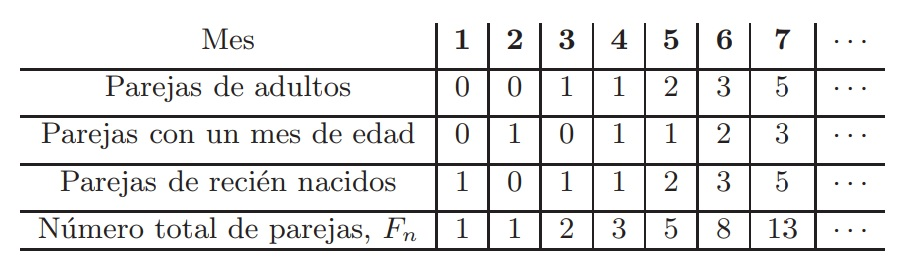
\includegraphics[scale=0.5]{y.jpg}
\end{figure}

De éstas hay tantas como parejas adultas hubiera en el mes $n$. Y a su vez, tantas como parejas en el mes $n-2$ (pues se tardan dos meses en ser adulto). En total, para cada $n \geq 3$,
$$F_n = F_{n-1} + F_{n-2}; \textit{ \qquad la ecuación de Fibonacci.}$$
Si definimos $F_0 = 0$, la ecuación de recurrencia es válida para cada $n \geq 2$. En lo sucesivo reservaremos el nombre de $F_n$ para los números siguientes:\\


Definición: La sucesión de números de Fibonacci $(F_n)$ cumple, para cada $n \geq 2$, que
$$F_n=F_{n-1} + F_{n-2} \textit{\qquad (la ecuación de Fibonacci)}$$
junto con las condiciones iniciales $F_0=0$, $F_1=1$. Los primeros términos de esta sucesión son

\begin{figure}[h]
    \centering
    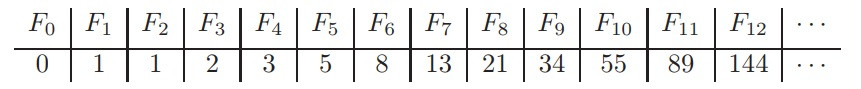
\includegraphics[scale=0.5]{x.jpg}
\end{figure}

la ecuación característica correspondiente es $r^2 - r -1 =0$, cuyas soluciones son como ya sabemos, $r_1 = (1 + \sqrt{5})/2$ y $r_2 = (1 - \sqrt{5})/2$; así que la solución general de la ecuación de Fibonacci es 

$$A (\frac{1 + \sqrt{5}}{2})^n + B(\frac{1-\sqrt{5}}{2})^n$$

En esta fórmula tenemos codificadas todas las soluciones de la ecuación de Fibonacci. Queda determinar los valores de A y B que corresponden a la sucesión que nos incumbe, la que tiene como valores iniciales 0 y 1. Sólo hay que escribir los casos $n=0$ y $n=1$ de la fórmula y resolver el siste,a de ecuaciones correspondiente 

\begin{itemize}
    \item $0 = F_0 = A + B$
    \item $1 = F_1 = A (\frac{1 + \sqrt{5}}{2}) + B(\frac{1-\sqrt{5}}{2})$
\end{itemize}

$\Rightarrow A = \frac{1}{\sqrt{5}} \textit{ y } B = -\frac{1}{\sqrt{5}}$\\

De manera que el n-ésimo número de Fibonacci se puede escribir como:
$$F_n = \frac{1}{\sqrt{5}}(\frac{1 + \sqrt{5}}{2})^n  -\frac{1}{\sqrt{5}}(\frac{1-\sqrt{5}}{2})^n$$














\end{document}
